\chapter{Stand van zaken}
\label{ch:stand-van-zaken}

% Tip: Begin elk hoofdstuk met een paragraaf inleiding die beschrijft hoe
% dit hoofdstuk past binnen het geheel van de bachelorproef. Geef in het
% bijzonder aan wat de link is met het vorige en volgende hoofdstuk.

% Pas na deze inleidende paragraaf komt de eerste sectiehoofding.

%Dit hoofdstuk bevat je literatuurstudie. De inhoud gaat verder op de inleiding, maar zal het onderwerp van de bachelorproef *diepgaand* uitspitten. De bedoeling is dat de lezer na lezing van dit hoofdstuk helemaal op de hoogte is van de huidige stand van zaken (state-of-the-art) in het onderzoeksdomein. Iemand die niet vertrouwd is met het onderwerp, weet er nu voldoende om de rest van het verhaal te kunnen volgen, zonder dat die er nog andere informatie moet over opzoeken \autocite{Pollefliet2011}.

%Je verwijst bij elke bewering die je doet, vakterm die je introduceert, enz. naar je bronnen. In \LaTeX{} kan dat met het commando \texttt{$\backslash${textcite\{\}}} of \texttt{$\backslash${autocite\{\}}}. Als argument van het commando geef je de ``sleutel'' van een ``record'' in een bibliografische databank in het Bib\TeX{}-formaat (een tekstbestand). Als je expliciet naar de auteur verwijst in de zin, gebruik je \texttt{$\backslash${}textcite\{\}}.
%Soms wil je de auteur niet expliciet vernoemen, dan gebruik je \texttt{$\backslash${}autocite\{\}}. In de volgende paragraaf een voorbeeld van elk.

%\textcite{Knuth1998} schreef een van de standaardwerken over sorteer- en zoekalgoritmen. Experten zijn het erover eens dat cloud computing een interessante opportuniteit vormen, zowel voor gebruikers als voor dienstverleners op vlak van informatietechnologie~\autocite{Creeger2009}.

%proberen meer in detail te treden per aangehaalde case

Tegenwoordig is artificiële intelligentie niet meer weg te denken uit onze maatschappij. Denk hierbij maar aan zelfrijdende auto’s of robotstofzuigers die weten waar het vuil is. Naast deze reeds bekendere voorbeelden, kan je met AI nog veel meer doen. Denk hierbij maar aan spraak- en tekstherkenning. Een voorbeeld hiervan is het al sprekend ingeven van zoekopdrachten op Google. Maar bestaat er ook een mogelijkheid om op deze manier, dus via spraak- of tekstherkenning, code te laten genereren?

Verscheidene bedrijven en organisaties zoals Google en Microsoft experimenteren met code generatie door middel van AI. Meestal gaat het hierbij over de generatie van SQL-query's, maar in de toekomst zou het misschien ook mogelijk zijn om bijvoorbeeld Java-code te laten genereren. 

\textbf{In deze sectie wordt het gedeelte binnen de AI besproken dat generatie van code mogelijk maakt.}
\section{Neurale netwerken}

Voor de generatie van code wordt er gebruik gemaakt van artificiële intelligentie, meer bepaald artificiële neurale netwerken. Maar wat zijn neurale netwerken? 

Wanneer iemand denkt aan neurale netwerken, wordt er meer bepaald gedacht aan het menselijke brein. Het menselijk brein bestaat uit een groot aantal neuronen. Deze neuronen werken samen door middel van elektrochemische signalen. Bij artificiële neurale netwerken probeert men alle kenmerken van een menselijk neuron samen te voegen in een wiskundig model. Over artificiële neurale netwerken valt er nog meer te lezen in de Hogeschool Cursus AI door \textcite{cursusAI} en in het artikel van \textcite{techpulse}.

Hoe werken artificiële neurale netwerken nu eigenlijk? 

Neurale netwerken worden getraind om te kunnen werken. Denk bijvoorbeeld aan het herkennen van nummers uit een lijst. Of zoals Facebook, die gezichten op foto’s herkend en vraagt om eventueel deze herkende mensen te taggen in de bewuste foto’s. 

Het voorbeeld dat wordt omschreven in het artikel op de website van tweakers (\textcite{tweakers}) gaat over het herkennen van handgeschreven getallen uit een foto. Deze foto of afbeelding (meestal 28 bij 28 pixels) wordt gebruikt als input voor het neurale netwerk. In de datasets die gebruikt worden voor het netwerk te trainen, zitten er ook afbeeldingen van 28 bij 28 pixels met handgeschreven cijfers op. De mens herkent makkelijk de cijfers in de afbeeldingen, door te kijken naar de grijswaarden in de pixels. Het neurale netwerk moet wel gaan rekenen, daarom worden aan alle ingaven (28 x 28 = 784) een waarde tussen 0 en 1 gegeven. Een neuraal netwerk is NIET binair, maar wel analoog. 

De data uit deze eerste laag neuronen, wordt doorgestuurd naar de tweede, verborgen, laag. Dit is een veel kleinere laag neuronen. In deze laag wordt er een bepaald gewicht gegeven aan de data van de input grijswaarden. De data uit de tweede laag krijgt dus ook weer een waarde tussen 0 en 1. Deze waarden worden dan doorgegeven aan de uitvoer neuronen. Het neuron dat het dichtste aanleunt tegen 1, geeft het cijfer aan dat het net “gezien” zou hebben. 

Een neuraal netwerk zou ook kunnen bestaan uit meerdere lagen neuronen. Voor de simpliciteit werd in dit voorbeeld maar één tussenlaag gebruikt.

Maar hoe worden neurale netwerken nu getraind? Voor het trainen van een neuraal netwerk, kan men één van de volgende vijf optimalisatiealgoritmen toepassen, welke beschreven zijn door \textcite{neuraldesigners}.

\begin{description}
	\item[Gradient Descent] Gradient Descent is het makkelijkste algoritme voor het trainen van een neuraal netwerk. Het is een eerste orde iteratief optimalisatie algoritme voor het vinden van een minimum van een functie. Door eerst voorwaartse propagatie uit te voeren en daarna achterwaartse propagatie, kan men de gradiënt berekenen. Het is wel de bedoeling dat de gehele training dataset onderzocht wordt. Door het uitvoeren van het gradiënt descent algoritme, kan men al een idee krijgen in welke richting de gewichten zich zouden aanpassen.
	\item[Methode van Newton] Gradiënt Descent is dan wel een eerste orde algoritme, de methode van Newton is een tweede orde algoritme. Het maakt gebruik van de Hessiaan\footnote{Dit is een matrix van de tweede orde partiële afgeleiden van een functie.} van de te minimaliseren functie. Deze functie wordt gebruikt om een betere trainingsrichting te vinden door de tweede orde afgeleiden van de verliesfunctie te gebruiken.
	\item[Conjugate gradient] De conjugate gradiënt is een vorm tussen de gradiënt descent en de methode van Newton. Via deze methode is het mogelijk om de normaal gezien langzame convergentie te versnellen (dit is zo bij gradiënt descent). Daarnaast wordt het werken met de Hessiaan matrix en alle andere benodigdheden van de methode van Newton ook vermeden.
	\item[Quasi-Newton-methode] De methode van Newton is duur in uitvoer. Er zijn veel bewerkingen nodig om voor die methode alles te berekenen. De quasi-Newton methode is een beter alternatief. Het is ontwikkeld om een antwoord te bieden alle nadelen van de methode van Newton. Bij deze methode wordt er per iteratie van het algoritme, een benadering gegeven op de inverse Hessiaan. Hiervoor worden enkel de eerste afgeleiden van de verliesfunctie gebruikt.
	\item[Het algoritme van Levenberg-Marquardt] Dit algoritme is speciaal ontworpen om te werken met verliesfuncties die de vorm aannemen van een som kwadratische fouten. In plaats van de Hessiaan-matrix te gebruiken, wordt er gebruik gemaakt van de Jacobi-matrix\footnote{De Jacobi-matrix van een functie is de matrix van de eerste-orde partiële afgeleiden van een functie.}.
\end{description}

Neurale netwerken zijn belangrijk voor het genereren van code uit tekst of uit natuurlijke taal. Deze neurale netwerken worden getraind om woorden te herkennen uit de gestelde vragen. Door middel van die woorden wordt er via allerhande mechanismen en algoritmen code gegenereerd.

\textbf{In de volgende secties worden er een aantal cases besproken waarbij programma's kunnen gegenereerd worden door middel van onder andere neurale netwerken. Hierbij kan er eventueel een onderscheid gemaakt worden tussen algoritmen die instaan voor de generatie van programma's, macchine learning en de generatie van SQL-query's.}

\section{Programma generatie}

\subsection{Microsoft DeepCoder}

In samenwerking met de universiteit van Cambridge, ontwikkelde Microsoft een mechanisme voor het “zelf schrijven van code”. Hierbij werd gebruik gemaakt van artificiële intelligentie en program synthesis. Het mechanisme kreeg de naam DeepCoder. Dat schrijft \textcite{DeepCoder} in een artikel op LinkedIn.

Met DeepCoder zouden mensen, ook al hebben ze geen enkele programmeerachtergrond, werkende code kunnen laten schrijven binnen een paar seconden. DeepCoder kan nu al gebruikt worden voor basis problemen op te lossen.

DeepCoder maakt gebruik van Program Synthesis, waarbij DeepCoder eigenlijk lijnen code “steelt” van werkende software. Daarnaast wordt er bruikbare code gezocht op websites zoals StackOverflow om te gebruiken in de te schrijven code. Eigenlijk volgt Program Synthesis de manier van werken van een programmeur (code opzoeken op het internet), maar doet dat veel sneller. Dit wordt onder andere vermeld in het artikel van \textcite{techcrunch} en het artikel van \textcite{NewScientist}.

DeepCoder is eigenlijk een implementatie van Program Synthesis. In de paper van \textcite{deepcoderpaper} wordt dit mechanisme \textit{Learning Inductive Program Synthesis (LIPS)} genoemd. Voor DeepCoder kunnen volgende componenten beschreven worden:
\begin{description}
	\item[Domein Specifieke Taal (DSL) en attributen] Er dient een DSL te worden gekozen die high-level constructies bevat die allemaal voorkomen in een overgrote meerderheid van de programma's. Tegelijkertijd dienen deze constructies algemeen genoeg te zijn, opdat het voorspellen van hun voorkomen door middel van input-outputvoorbeelden succesvol kan aangeleerd worden.
	\item[Data generatie] Wanneer er een geldige invoer voor een programma dient gegenereert te worden, dient er een beperking op de uitgangswaarde te worden afgedwongen. Deze beperking stelt dat gehele getallen dienen begrenst te worden tot een vooraf bepaald bereik. Nadien worden deze beperkingen achterwaarts verspreid door het programma. Als resultaat wordt er een bereik van geldige waarden voor elke invoer verkregen.
	\item[Machine Learning Model] Het doel van DeepCoder is om patronen te herkennen in input-outputvoorbeelden. Deze worden dan ook gebruikt om de aan- of afwezigheid van individuele functies te voorspellen. Er wordt gebruik gemaakt van neurale netwerken voor moddeleren van de toewijzing van de input-outputvoorbeelden aan de attributen. Deze netwerken bestaan uit twee onderdelen:
	\begin{itemize}
		\item Encoder
		\item Decoder
	\end{itemize}
	\item[Zoekprocedures] Door middel van een neuraal netwerk wordt er gezocht naar programma's die consistent zijn met de input-outputvoorbeelden. Het voorspellen van broncode wordt niet direct gedaan. Volgende zoektechnieken worden toegepast voor dit tot een goed einde te brengen:
	\begin{itemize}
		\item Depth-first search (DFS): Zoekalgoritme voor het doorzoeken van een boom of graaf. Er wordt gestart bij de wortel om dan een tak te kiezen om deze dan verder te onderzoeken, zonder terug te keren naar de vorige stappen.
		\item Sorteren en toevoegen enumeratie:  Dit is een manier om de voorspelde kansen op functies in een enumeratieve zoekprocedure te gebruiken. Hierbij wordt er DFS toegepast op de actieve functieset. Indien bijvoorbeeld een zoekopdracht mislukt, wordt de zoekopdracht opnieuw gestart met een grotere actieve set. Deze set werd uitgebreid met de volgende meest waarschijnlijke functie.
		\item Sketch: Een succesvol SMT-gebaseerd programma welke kan gebruikt worden programma's te doorzoeken om zo "gaten" in de onvolledige broncode in te vullen. Zo kan voldaan worden aan de opgegeven vereisten.Er kan voor dit mechanisme gebruik gemaakt worden van "Sorteren en Toevoegen"-mechanisme. De mogelijkheden voor elk "gat" kunnen beperkt worden tot de huidige actieve set.
	\end{itemize}
\end{description}

Programmeurs hoeven geen schrik te hebben voor hun job. DeepCoder zou in de toekomst kunnen gebruikt worden om het vuile, herhalende werk op te knappen. Programmeurs zouden de eerder moeilijke taken uitvoeren.

\subsection{Primary Objects - AI Programmer}

AI Programmer is het eerste machine learning systeem dat in staat is om volledige code te genereren. De mens dient maar weinig hulp eraan te bieden om het te doen slagen. Door middel van artificiële intelligentie en enkele genetische algoritmes, is AI Programmer in staat om een aantal kleine programmatjes te produceren (zie ook de Github-repository van \textcite{github} en de tutorial van \textcite{primaryObject} op de website van PrimaryObjects).

AI Programmer is een zelflerend mechanisme. Het is een AI genetisch algoritme dat zichzelf altijd tracht te verbeteren. Het achterliggende idee voor de ontwikkeling van dit mechanisme, is het mogelijk maken dat een computer allerlei soorten programma's kan creëren. Het ultieme doel is om computerprogramma’s te genereren voor het oplossen van problemen.

In de paper van \textcite{aiProgrammer} wordt het volledige model voorgesteld. In figuur \ref{fig:aiprog} wordt het ontwerp van AI Programmer (door Salesforce) voorgesteld. Het mechanisme maakt gebruik van een typeloze programmeertaal. Deze programmeertaal bevat maar acht instructies om de generatie van software door middel van AI Programmer te sturen. De acht instructies zijn: '<' , '>' , '+' , '-' , '.' , ',' , '[' en ']'. Deze manier van werken brengt een aantal voordelen met zich mee, alsook een aantal aanpassingen aan de taal om alles te kunnen integreren:
\begin{description}
	\item[Turing Compleet] Door AI Programmer gegenereerde programma’s zijn in theorie in staat om alle te voldoen aan alle taken die men zou willen of kunnen uitvoeren met een computer.
	\item[GA-Engine en Uniforme Gene Distributions] Het genetisch algoritme (GA) mechanisme van AI Programmer toont de instructies van de gegenereerde programma’s als een array van floating point waarden. Wanneer dit beschouwd wordt als een eenheid, is dit zijn genoom. Een individuele locatie binnen een bepaald genoom staat bekend als een gen (gene). Een bepaald gen binnen een genoom komt overeen met één van de acht opgegeven instructies. Tijdens het uitvoeren van dit algoritme wordt er aan elke instructie een bepaald bereik waartussen de genwaarde kan vallen. Dit gebeurt via een continue uniforme verdeling (de grootte van het bereik is voor elke instructie even groot). De reden om dit zo te doen, is het feit dat iedere instructie een willekeurige kans had om op iedere mogelijke locatie in een gensequentie te worden gekozen (wanneer willekeur nodig is).
	\item[Vereenvoudige set van instructies]  Een vereenvoudigde instructieset zorgt ervoor dat de zoekruimte waarin doelprogrammacode dient gevonden te worden verkleint. Het is belangrijk te onthouden dat AI Programmer bedoeld is voor ontwikkelaars voor algemene doeleinden. Het beperken van de instructies (op acht instructies) kan ervoor zorgen dat dit mechanisme binnen een redelijke tijd uitgevoerd kan worden op basis hardware.
\end{description}

\begin{figure}[htb]
	\centering
	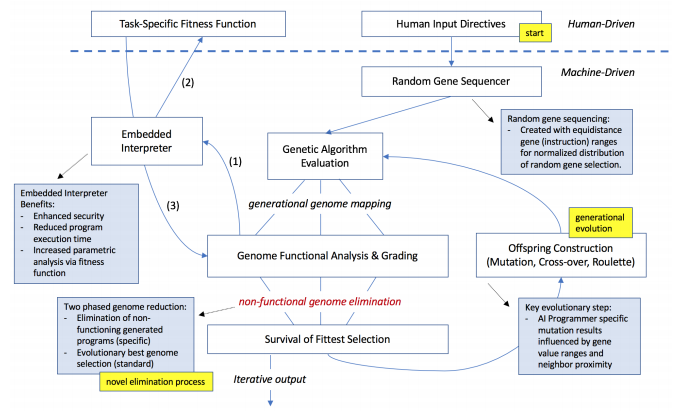
\includegraphics[width=0.80\textwidth]{img/aiprogmodel}
	\caption[AI Programmer Model]{AI Programmer - Softwarearchitectuur}
	\label{fig:aiprog}
\end{figure}
\break 

AI Programmer is een genetisch algoritme. Voor het genereren van een programma via zo'n algoritme, moet er eerst een genoom gecreëerd worden. In de biologie wordt een genoom beschreven als de complete genetische samenstelling van een organisme, cel of virus. In deze context wordt een genoom ongeveer gelijkaardig beschreven. Zoals eerder beschreven, is een genoom (bij AI Programmer) een array van floating point waarden. 

Wanneer zo’n genoom is aangemaakt, wordt dit omgezet naar een overeenkomstig programma. Na deze omzetting wordt het programma uitgevoerd en aan dat resulterend programma wordt er een fitnessscore toegekend. Hoe beter het programma overeenkomt met het gevraagde, hoe groter de fitnessscore. Hierdoor is de kans groter dat het programma doorgaat naar een volgende evolutionaire generatie. Bij elke generatie maakt AI Programmer gebruik van willekeurige selectie, cross-over en mutatie. Hierdoor worden er telkens programma’s gegenereerd met kleine “verstoringen” die mogelijk betere genomen bevatten dan hun parents voor het oplossen van de doeltaak.

Om een genetisch algoritme te kunnen gebruiken, is een fitnesstest nodig om uit te maken hoe  goed een bepaalde oplossing overeenkomt met het beoogde doelprogramma. Dit concept komt overeen met het test-driven ontwikkelen van programma’s. Wanneer alle testen slagen, is een programma pas correct. Bij AI Programmer bezit de fitnesstest meestal een reeks controles voor verschillende scenario’s. Deze begeleiden de genoom selectie. Indien de programma’s goed evalueren op de testsuite, worden deze behouden.

Een gegenereerd programma moet dan ook uitgevoerd kunnen worden. Daarna wordt het beoordeeld aan de hand van fitnesstests. Uitvoeringen van de gegenereerde programma’s kunnen altijd beveiligingsrisico’s of prestatieverminderingen met zich meebrengen. Met dit in het achterhoofd te houden alsook de behoefte aan een complexe fitnessfunctie, ontwikkelde de onderzoekers van AI Programmer een eigen soort tolk (interpreter). Dit mechanisme zit ingebouwd in AI Programmer en biedt een veilige, efficiënte en GA-geschikte uitvoeringsomgeving. Zo’n interpreter brengt ook voordelen en uitdagingen met zich mee:

\begin{itemize}
	\item Uitvoering in een gecontroleerde omgeving
	\item Beëindigen van oneindige lussen
	\item Simulatie van complexe instructies
\end{itemize}

Er worden in de paper ook een aantal testen beschreven. Zo hebben de onderzoekers een aantal programma’s laten genereren. Deze programma’s gingen van begroetingen tot conversies van invoergegevens. In tabel \ref{table:aiprog} wordt er een overzicht getoond van de gegenereerde programma’s, alsook de tijd die nodig was om deze te produceren en het totaal aantal evolutionaire generaties welke gebruikt werden voor het builden van de programma’s. Het is belangrijk te weten dat, door de variatie in genoomgrootte en de berekening van de fitnessfunctie welke voor elk programma uniek is, het aantal evolutionaire generaties \textbf{NIET} gelijk is aan de totale computertijd voor de generatie van het programma.

\begin{table}[htb]
	\centering
	\begin{tabular}{lll}
		\hline
		Naam                        & Duur (s) & Generaties \\ \hline
		hi                          & 52       & 5700       \\
		Hi!                         & 7644     & 1219400    \\
		hello                       & 1713     & 252000     \\
		hello world                 & 7702     & 580900     \\
		reddit                      & 1362     & 195000     \\
		Keep Calm Keep Coding       & 944      & 21400      \\
		I love all humans           & 36000    & 6057200    \\
		hello\{user\}               & 1793     & 42800      \\
		Addition                    & 2698     & 92400      \\
		Substraction                & 4305     & 177900     \\
		Multiply x2                 & 6353     & 242000     \\
		Multiply x3                 & 5165     & 87200      \\
		XOR                         & 2095     & 146400     \\
		Fibonacci                   & 21862    & 151900     \\
		If/then conditionals        & 8313     & 46200      \\
		cats are evil               & 10209    & 814400     \\
		Bottles of Beer on the Wall & 2957     & 61400      \\
		Reverse string              & 49       & 2600       \\
		CSV parse                   & 173      & 9000       \\
		Extract in quotes           & 6478     & 212100     \\
		Extract in quotes 2         & 9996     & 188400     \\
		Trim left of quote          & 9030     & 341700     \\
		XML to JSON                 & 6866     & 820900     \\
		Warning countdown           & 48       & 900       
	\end{tabular}
	\caption{Resultaten AI Programmer}
	\label{table:aiprog}
\end{table}

De programmeerwereld blijft zichzelf altijd heruitvinden. Software en hardware wordt altijd complexer. De software-ontwikkeling zal de capaciteit van programmeurs binnenkort overstijgen. Naarmate deze tijd nadert, zullen programmeurs nood hebben aan assistentie van automatische softwareontwikkelingsalgoritmen. Hiervoor kan AI Programmer dan een mogelijke oplossing zijn.

\section{Machine Learning}

\subsection{Google AutoML}

Naast Microsoft is Google ook bezig met het ontwikkelen van een mechanisme waarbij artificiële intelligentie wordt gebruikt voor de generatie van code. Dit onder de naam “Google AutoML”. Eén van de belangrijkste kenmerken van AutoML, is dat het mechanisme zichzelf altijd tracht te verbeteren. Het is nu al zo ver gekomen dat dit mechanisme betere code kan schrijven dan de programmeurs die het ontwikkeld hebben. Dit werd beschreven door \textcite{greene}.

Google ontwikkelde hun AutoML als oplossing voor het gebrek aan talent bij de AI-programmeurs. De vraag naar gespecialiseerde programmeurs is zo groot geworden, dat AutoML als oplossing werd aangereikt. 

Het systeem voert duizenden simulaties uit om te bepalen welke delen van de code kunnen worden verbeterd, de wijzigingen aan te brengen en de procesadvertentie oneindig door te zetten of totdat het doel is bereikt. 

AutoML Vision is de eerste service die uitgebracht werd voor het totale AutoML plaatje, zo meldt \textcite{automl}. Via AutoML Vision is het mogelijk om zaken te herkennen in foto’s van personen of dingen. Het is zeer eenvoudig om naar eigen nood modellen te trainen voor het herkennen van beelden. Binnenkort zal Google nog meerdere services toevoegen aan hun AutoML.

AutoML behoort tot Google Cloud. Eén van de features van dit mechanisme is dan ook dat het volledig is geïntegreerd met andere Google Cloud services. Het maakt de klant mogelijk om de volledige Cloud service van Google op een consistente manier te gebruiken. Trainingsgegevens kunnen makkelijk worden opgeslagen op de Google Cloud Storage, voorspellingen voor getrainde modellen (AutoML Vision) kunnen eenvoudigweg gegenereerd worden door de Vision API of door de voorspellingsservice van de Cloud ML Engine, \dots.

Volgens het artikel van \textcite{tc} meldt Google dat AutoML het enige systeem van zijn soort is die op dit moment op de markt is. Maar dat is niet zo! Er zijn op dit moment reeds gelijkaardige services beschikbaar. Clarif.ai is bijvoorbeeld zo’n service. Men is zelfs in staat om de vooraf gestelde visie, spraakherkenning en besluitvorming van de Cognitieve Services van Microsoft aan te passen.
 
AutoML is nog gloednieuw. Het is ongeveer een jaar geleden voorgesteld. Google verwacht dat AutoML de basis vormt voor de volgende generaties in machine-learning. AutoML is geen open source mechanisme, dit is enkel te gebruiken na het aanschaffen van een nodige licentie.

\section{SQL-generatie}

\subsection{Vierde generatie programmeertalen}

De volgende secties beschrijven algoritmen die SQL-query's trachten te genereren door middel van artificiële intelligentie en natuurlijke taal. Maar wat voor soort programmeertaal is SQL eigenlijk? Wel, SQL behoort tot de groep van de vierde generatie programmeertalen.

Maar wat is er zo speciaal aan deze generatie programmeertalen? Volgens \textcite{fourthgenpl} behoren de 4GL tot de talen die het dichtst aanleunen tegen de natuurlijke taal. Ze hebben het voordeel van onder andere sneller te kunnen verlopen en de kosten voor de ontwikkeling te verminderen.

Vierde generatie programmeertalen zijn de enige talen die vaak in contact komen met grote hoeveelheden aan data. Onder de vierde generatie programmeertalen kan je daarom volgende domeinen terugvinden:
\begin{itemize}
	\item Databasequery’s
	\item Rapporteringen
	\item Gegevensmanipulatie
	\item \dots
\end{itemize}

Het is dus via zo’n talen mogelijk om data op te vragen uit tabellen, deze aan te passen of mooi uit te schrijven in een rapport.

Naast SQL behoren onder andere volgende programmeertalen ook tot de vierde generatie: R, S, ABAP, Oracle Forms en Bizagi.

\subsection{Salesforce - Seq2SQL}
\label{sec:Salesforce - Seq2SQL}

Het Seq2SQL van Salesforce is een eerder concreet voorbeeld voor code generatie door middel van artificiële intelligentie. Seq2SQL is een mechanisme dat, door middel van AI en reïnforcement learning\footnote{Het is een mechanisme dat in staat is om uit eigen ervaringen te leren. Wanneer het mechanisme iets goed doet, wordt het hiervoor beloond. Het zal die stappen blijven uitvoeren waarvoor het de meeste beloningen heeft gekregen. Het doel is om het meeste beloningen te verkrijgen.}, gestructureerde SQL-query’s kan genereren. Hier werd grondig onderzoek naar gedaan. Dit valt allemaal te lezen in de paper, opgesteld door \textcite{seq2sqlPaper}.

Tegenwoordig wordt data bijna altijd opgeslagen in een relationale databank. Gegevens kunnen enkel via query’s, eigen aan de vooropgestelde SQL-syntax, opgehaald worden. Seq2SQL werkt anders.

Via dit model kunnen er vanuit natuurlijke taal, SQL-query’s gegenereerd worden. Hiervoor wordt gebruik gemaakt van neurale netwerken. Deze neurale netwerken worden zo geprogrammeerd dat deze gelijkaardig werken als het menselijke brein. 

Het Seq2SQL-model maakt volgens de paper (\textcite{seq2sqlPaper}) gebruik van het Seq2Seq-model. Volgens de basistheorie, beschreven door \textcite{drnn}, bestaat zo’n model uit 2 belangrijke onderdelen, een encoder en een decoder. Beiden zijn recurrente lagen van het neurale netwerk\footnote{De mogelijkheid om verder te bouwen op eerdere typen netwerken met ingangsvectoren van een vaste grootte en uitgangsvectoren – Definitie door \textcite{rnn}.}. Er wordt, door de encoder, een invoerreeks verwerkt tot een vaste representatie. De uitkomst van de encoder dient als context voor de decoder. Deze verwerkte informatie wordt hier dan gedecodeerd tot een bepaalde uitvoerreeks. In figuur \ref{fig:seq2seq} wordt er een visueel beeld gegeven van dit model. Dit voorbeeld wordt ook door \textcite{drnn} gegeven.

\begin{figure}[ht]
	\centering
	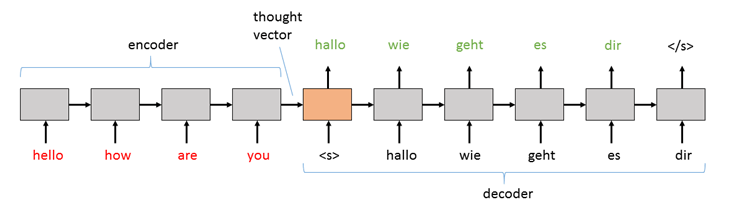
\includegraphics[width=0.80\textwidth]{img/Seq2Seq}
	\caption[Sequence-To-Sequence Model]{Sequence-To-Sequence Model}
	\label{fig:seq2seq}
\end{figure}

Een SQL-query bestaat meestal uit drie onderdelen. Als eerste component heeft u de aggregatie-operator (zoals COUNT en SUM). Dit geeft een samenvatting weer van de rijen die door de SQL-query worden aangeroepen. Ook kan het mogelijk zijn dat er geen operator meegegeven wordt. Het tweede component is de kolom waarop de query dient uitgevoerd te worden. Het derde en laatste component is de WHERE-clause. Dit geeft aan op welke rij(en) er dient gefilterd te worden. Seq2SQL zorgt ervoor dat een vraag direct in zo’n vorm kan gegoten worden (zie figuur \ref{fig:seq2sql}).

\begin{figure}[ht]
	\centering
	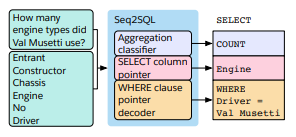
\includegraphics[width=0.80\textwidth]{img/seq2sqlmodel}
	\caption[Seq2SQL Model]{Seq2SQL Model}
	\label{fig:seq2sql}
\end{figure}

Het augmented pointer network is een zeer belangrijk netwerk voor Seq2SQL. Dit netwerk genereert woord voor woord de SQL-query van een invoerreeks. De uitkomst van dit netwerk mag dan wel een SQL-query zijn, maar dit is niet volledig volgens de reeds beschreven vorm. Daarvoor dient dan Seq2SQL. Eerst wordt door het netwerk de aggregatie-operator gezocht in de invoerreeks. Deze waarde kan eveneens null zijn, wanneer er geen aggregatie voorgeschreven is. Voor het volgende onderdeel zoekt het netwerk naar de kolom waarop het de query dient uit te voeren. Als laatste wordt via een pointer network gezocht naar de condities waarop eventueel gefilterd kan worden. De twee eerste componenten worden gesuperviseerd door middel van cross entropy\footnote{Cross entropy is het aantal bits dat nodig is om symbolen uit de verzameling p te encoderen, gebruik makend van de foutieve verzameling q – Definitie door \textcite{rdp}.} loss. Het derde component wordt getraind door middel van policy reïnforcement learning. Hiermee wordt de ongeordende aard van de query aangepakt.

Seq2SQL wordt in deze paper van \textcite{seq2sqlPaper} niet enkel theoretisch aangehaald. Er wordt ook een experiment beschreven waarbij het algoritme wordt uitgetest inzake performantie.  Voor deze experimenten werd gebruik gemaakt van de WikiSQL-dataset (\textcite{wikisql}). Deze dataset is een verzameling van de meest gebruikte SQL-query’s die gebruikt werden tijdens de zoekopdrachten op Wikipedia. WikiSQL wordt gebruikt om het model van Seq2SQL te trainen. De broncode kan gevonden worden op de Github-repository van \textcite{seq2sql}.

Uit de resultaten van de uitgevoerde experimenten blijkt dat de performantie het grootst is bij het uitvoeren van het volledige Seq2SQL algoritme. Dit dus met het toepassen van reïnforcement learning. Seq2SQL zonder het gebruik van reïnforcement learning levert een performantie op die zo’n 2,7\% lager is dan het volledige model. De volledige resultaten worden voorgesteld in tabel \ref{table:seq2sqltab}.

Enkele conclusies die hierbij getrokken kunnen worden:
\begin{itemize}
	\item Het beperken van de uitvoerruimte leidt tot meer nauwkeurige omstandigheden.
	\item Het toepassen van de juiste SQL-structuur zorgt voor minder ongeldige queries.
	\item Reïnforcement learning zorgt ervoor dat de WHERE-clauses van een goede kwaliteit zijn.
\end{itemize}

\begin{table}[ht]
	\centering
	\begin{tabular}{lllll}
		\hline
		Model                & Dev Acc\textsubscript{lf}       & Dev Accex       & Test Acc\textsubscript{lf}      & Test Accex      \\ \hline
		Attentional Seq2Seq  & 23.3\%          & 37.0\%          & 23.4\%          & 35.9\%          \\
		Aug. Pointer Network & 44.1\%          & 53.8\%          & 42.8\%          & 52.8\%          \\ \hline
		Seq2SQL (no RL)      & 47.7\%          & 57.9\%          & 47.2\%          & 57.6\%          \\
		\textbf{Seq2SQL}     & \textbf{49.8\%} & \textbf{60.7\%} & \textbf{49.2\%} & \textbf{60.3\%}
	\end{tabular}
	\caption{Resultaten Seq2SQL}
	\label{table:seq2sqltab}
\end{table} 

\subsection{SQLNet}
\label{sec:SQLNet}

Naast Seq2SQL, bestaat er ook SQLNet. Dit mechanisme werkt op een ongeveer gelijkaardige manier als Seq2SQL, maar hier wordt geen reïnforcement learning toegepast. De huidige manier van werken (het belonen van het model) is niet eerder beperkt. Daarom is het nodig dat er verandering komt. SQLNet komt hier dus met de oplossing.

SQLNet werkt volgens een schetsmatige benadering waarbij een schets een afhankelijkheidsgrafiek bevat. Op die manier kan een voorspelling gedaan worden wanneer eerdere, afhankelijke voorspellingen in overweging te nemen. 

Maar hoe werkt dat nu precies? SQLNet wordt in de paper van \textcite{sqlnetPaper} grondig voorgesteld. Het basisidee van SQLNet is het gebruik van een schetsmatige voorstelling die overeenkomt met de SQL-grammatica. Het mechanisme dient enkel de plaatsen in de schets op te vullen. De schets is zo opgebouwd, dat het mogelijk is om alle soorten query’s te kunnen genereren.

Het gebruikmaken van zo’n schets heeft als voordeel dat de orderaangelegenheden die kunnen voorkomen in een sequence-to-sequence-model (zie  sectie \ref{sec:Salesforce - Seq2SQL} ) te voorkomen. Dit komt omdat de schets de afhankelijkheid van de voorspellingen vastlegt. Om te kunnen voldoen aan deze schets, wordt er gebruik gemaakt van twee technieken: sequence-to-set en column attention. Alle mogelijke technieken worden gebruikt zodat er een SQLNet neuraal netwerk wordt gecreëerd waarbij het mogelijk is om een SQL-query te genereren vanuit een natuurlijke taalvraag en een tabelschema.

De eerste stap voor het uitvoeren van het SQLNet-algoritme, is het opstellen van de schets. Dit gebeurd door middel van de zogenaamde “sketch-based query synthese”. De SQL sleutelwoorden worden al gegeven. Dit zijn SELECT, WHERE en AND. In de paper wordt volgende figuur getoond (figuur \ref{fig:sqlnet}a). Hierin kan er gezien worden dat deze woorden reeds ingevuld zijn. De operatoren die starten met “\$” dienen gevonden te worden. Enkel en alleen de AND-clausule dient niet ingevuld te worden. Om dit duidelijk te maken, wordt er gebruik gemaakt van een reguliere expressie (“()*”). In figuur \ref{fig:sqlnet}b kan de zogenaamde afhankelijkheidsgrafiek teruggevonden worden. De nog te vinden operatoren worden hier voorgesteld in kaders. Elke afhankelijkheid wordt voorgesteld door middel van een gerichte pijlen. Deze pijlen geven de afhankelijkheden weer ten opzichte van zowel de kolom als de gestelde vraag. Het model kan gezien worden als een grafisch model op basis van de afhankelijkheidsgrafiek. Ook het probleem van de vraagsynthese kan gezien worden als een gevolgtrekkingsprobleem in deze grafiek. Als besluit voor dit onderdeel, kan men zeggen dat de voorspelling van een beperking onafhankelijk is van een andere voorspelling. Deze benadering brengt dus een oplossing voor het “order-zaken”-probleem bij een sequence-to-sequence model.

\begin{figure}[ht]
	\centering
	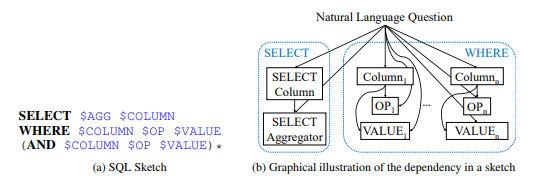
\includegraphics[width=0.80\textwidth]{img/sqlnetmodel}
	\caption[SQLNet Model]{Syntax van de schets en zijn afhankelijkheden}
	\label{fig:sqlnet}
\end{figure}

Er werd al gesproken over de sequence-to-set voorspelling en de column attention, maar wat is dit nu? In de paper van \textcite{sqlnetPaper} wordt het voorspellen van de WHERE-kolom gebruikt als voorbeeld om dit uit te leggen. De kolommen in de WHERE-component zijn een subset van een reeks kolomnamen. Sequence-to-set voorspellingen is het voorspellen van de belanghebbende kolomnamen die in deze subset moeten weergegeven worden. Column attention is een speciale vorm van het generieke aandachtsmechanisme om te berekenen op welke kolommen de aandacht moet gevestigd worden. 

Het SQLNet model bestaat uit het voorspellen van het SELECT-statement en het voorspellen van het WHERE-statement. Beiden worden gescheiden van elkaar voorspelt:
\begin{description}
	\item[WHERE] Het voorspellen van de WHERE-clausule is het moeilijkste van het hele proces. Het maakt gebruik van het sequence-to-set-mechanisme om eerst en vooral de set van kolommen welke nodig zijn voor de WHERE-clausule te voorspellen. Voor elke kolom wordt dan een constraint gegenereert door het voorspellen van de OP- en VALUE-slots 
	\footnote{
		\begin{description}
			\item[OP-slot] De waarde in het OP-slot moet berekend of voorspelt worden voor elke kolom in de WHERE-clausule. Voor het voorspellen van deze waarde heeft het model 3 keuzes, namelijk:
			\begin{itemize}
				\item =
				\item >
				\item <
			\end{itemize}
			\item[VALUE-slot] Hiervoor moet er een substring van de taalvraag voorspelt worden. Aangezien de volgorde van de tokens  in de substring van belang is, maakt het systeem gebruik van het sequence-to-sequence model (zie sectie \ref{sec:Salesforce - Seq2SQL}) om de substring te voorspellen. Het genereren van het VALUE-slot stopt wanneer het (END)-token is voorspelt. Dat token komt voor in elke vraag.
		\end{description}
	}.
	\item[SELECT] Een SELECT-statement bestaat meestal uit een aggregatieparameter en een kolomnaam. Deze kolomnaam voorspellen is gelijkaardig aan het voorspellen van de kolommen die gebruikt worden bij een WHERE-statement. Het grootste verschil tussen beiden is dat voor een SELECT-statement maar één kolom moet voorspelt worden.
\end{description}

Net als bij Seq2SQL wordt voor dit model gebruik gemaakt van de WikiSQL-dataset voor het uitvoeren van de experimenten en het trainen van het model. Zo kan er bewezen worden dat door het uitvoeren van het SQLNet-mechanisme, 9 tot 13 procent beter werkt dan een ander mechanisme. De volledige source code kan gevonden worden op de Github-repository van \textcite{sqlnet}.

\subsection{Algoritme voor transformatie van tekst naar SQL-query's (NLIDBS)}

Zoals vermeld bij Seq2SQL, worden grote hoeveelheden data opgeslagen in relationele databanken. Een groot nadeel hierbij is dat de meeste mensen de kennis niet hebben inzake SQL om te communiceren met de databank. Een oplossing hiervoor zou zijn dat mensen in hun eigen taal zouden kunnen communiceren met de databank. Deze oplossing staat beschreven in het artikel van \textcite{nlidbs}.

Onderzoekers hebben een intelligente interface ontwikkeld die natuurlijke taalquery’s (zoals “Geef een lijst van de laatste 5 presidenten van Amerika.”) omzet naar SQL-query’s. Er wordt hier gebruik gemaakt van semantische matchingtechnieken. Hierbij wordt er rekening gehouden met de betekenis van de woorden in de opgegeven zoekstring. 

Er worden negen stappen uitgevoerd om tot de juiste query te komen. Door deze query dan uit te voeren op de databank, komt het juiste antwoord naar boven. Hieronder worden de stappen voorgesteld die beschreven staan in het artikel van \textcite{nlidbs}:

\begin{description}
	\item[Grafische User Interface] Via de GUI biedt de gebruiker de mogelijkheid aan om een query in te geven. Deze query wordt als een natuurlijke taalvraag ingegeven. Deze vraag wordt verder gebruikt tijdens het gehele algoritme.
	\item[Omzetten hoofd- naar kleine letters] Elk woord in de vraag wordt bekeken om eventueel de hoofdletters om te zetten naar kleine letters.
	\item[Zin opdelen in aparte woorden] De volledige vraag wordt opgedeeld in aparte woorden. Elk woord krijgt hier nu een eigen order-nummer.
	\item[Verwijderen van extra/stopwoorden] Alle woorden die niet nodig zijn worden uit de vraag weggelaten. Enkel de woorden die database-gerelateerd zijn worden geselecteerd. Alle geïdentificeerde SQL-elementen worden in arrays opgeslagen.
	\item[Classificatie van (voor)naam-/werkwoorden] De overgebleven woorden worden geclassificeerd. Voornaamwoorden krijgen een tag “voornaamwoord”, zelfstandige naamwoorden krijgen de tag “zelfstandige naamwoorden” en werkwoorden de tag “werkwoorden”. Zo worden de overgebleven woorden opgedeeld in klassen.
	\item[Classificatie van relaties, attributen en clausules] Op basis van de gelabelde elementen worden relaties, attributen en clausules geclassificeerd. Daarnaast worden integers en strings van elkaar gescheiden voor het vormen van de clausules.
	\item[Verwijderen van dubbelzinnigheid] De dubbelzinnigheden die meerdere keren bestaan worden uit de vraag verwijderd. Daarna wordt het meest geschikte attribuut geëxtraheerd en wordt het samen let de relatie in kaart gebracht.
	\item[Genereren van een query] Na allerhande operaties wordt de gevraagde query gegenereerd.
	\item[Resultaat] De gegenereerde query wordt uitgevoerd op de testdataset. De interface toont dan de verkregen resultaten aan de gebruiker.
\end{description}

Het volledige proces wordt voorgesteld in figuur \ref{fig:nlidbs}, verkregen uit het artikel van \textcite{nlidbs}.

\begin{figure}[ht]
	\centering
	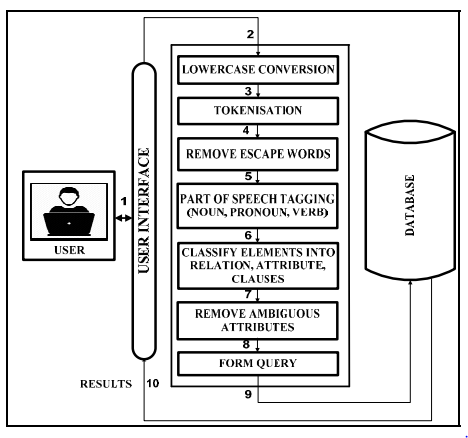
\includegraphics[width=0.80\textwidth]{img/nlidbs}
	\caption[NLIDBS proces]{NLIDBS Process control flow diagram}
	\label{fig:nlidbs}
\end{figure}

Dit systeem werd geïmplementeerd in PHP, HTML, CSS en Javascript (als frontend), met een MySQL-databank als backend systeem.

Van het in het artikel beschreven algoritme is er helaas geen open source code teruggevonden. Wel bestaan er gelijkaardige Github-repositories waarbij er een mechanisme gebouwd wordt die dient als gebruikersinterface van een databank. Bij deze soort interfaces dient men een natuurlijke vraag in te geven. Een voorbeeld van zo'n Github-repository is de repository van \textcite{nlidb}.

\subsection{Microsoft Research - NL2Prog}

Eigenlijk is het doel van het onderzoek, beschreven in de paper NL2Prog, gelijkaardig aan het onderzoek uitgevoerd in Seq2SQL en in NLIDBS. De meeste mensen zijn niet in staat om via query's te communiceren met de databank wegens geen (of alleszins te weinig) programmeerkennis. De mens wil instaat zijn op een normale manier te kunnen communiceren met de databank, dus eigenlijk via hun eigen taal. Hiervoor probeert men een oplossing te bieden in de paper van \textcite{nl2prog}.		

Voor dit model wordt gebruik gemaakt van een deep sequence-to-sequence model. Hierbij wordt als decoder een eenvoudig type systeem van SQL-expressies gebruikt, welke gebruikt worden om de uitvoervoorspelling te structureren. Door middel van het type kopieert de decoder een mogelijke output van de inputstring. Dit met behulp van een op aandacht-gebaseerd kopieermechanisme, ofwel genereerd het een query vanuit een vast vocabulair.

Meer in detail: NL2Prog genereert SQL-query’s met behulp van een RNN-gebaseerd encoder-decoder model. Er wordt uitgegaan van het bekende ontwerp van een SQL-query. Dit om statisch het type van uitvoer van de decodeerstap te bepalen tijdens de generatie van een query. Zo weet men dat het derde woord in een query, na de aggregatieoperator, altijd een kolomnaam is. 

Tijdens het decoderen wordt statisch het type woord bepaald dat dient gegenereerd te worden. Dit gebeurt aan de hand van zijn decodering time stamp. Dan wordt er gebruik gemaakt van een gespecialiseerde decoder om de uitvoer te genereren. Wanneer er een kolomnaam of een constante dient gegenereerd te worden, wordt er gebruik gemaakt van een kopieermechanisme. Anders wordt de achterliggende status geprojecteerd naar een ingebouwd vocabulair om een ingebouwde SQL-operator te verkrijgen. Dit betekent op zijn beurt dat men enkel een kleine hoeveelheid vocabulair van de ingebouwde decoder dient te onderhouden voor elke operator.

\begin{description}
	\item[ENCODER] Dit is een bi-directioneel recurrent neuraal netwerk (RNN) welke gebruik maakt van Long Short-Term Memory eenheden \footnote{Long Short-Term Memory eenheden zijn bouwstenen van een RNN. Een LSTM bestaat uit een cel, een invoerpoort, een uitvoerpoort en een vergeetpoort. De cellen van zo’n geheugen zijn verantwoordelijk voor het onthouden van waarden op willekeurige tijdsintervallen. Alle soorten poorten kunnen aanzien worden als een conventioneel kunstmatig neuron. We kunnen ze voorstellen als regulators van de stroom van waarden die in de LSTM gaat.Dit is een bi-directioneel recurrent neuraal netwerk (RNN) welke gebruik maakt van Long Short-Term Memory cellen. Long Short-Term Memory eenheden zijn bouwstenen van een RNN. Een LSTM bestaat uit een cel, een invoerpoort, een uitvoerpoort en een vergeetpoort. De cellen van zo’n geheugen zijn verantwoordelijk voor het onthouden van waarden op willekeurige tijdsintervallen. Alle soorten poorten kunnen aanzien worden als een conventioneel kunstmatig neuron. We kunnen ze voorstellen als regulators van de stroom van waarden die in de LSTM gaat.}. Een concatenatie van de table header (i.e. de kolomnamen) van de gevraagde tabel en de gebruikersvraag wordt gebruikt als invoertoken. Deze concatenatie laat het model toe te leren hoe een gezamenlijke representatie voor de beide kolommen en de invoervraag kan worden berekend.
	\begin{description}
		\item[Token Embedding] Een invoervraag bestaat meestal uit meerdere verschillende tokens. Om dit grote aantal verschillende tokens te verwerken, combineren we een pre-trained character n-gram embedding met een pre-trained global word embedding. 
		\item[Bidirectionele RNN] De embedded tokens worden toegevoegd aan de RNN, welke bestaat uit LSTM eenheden. Hieruit wordt er een sequentie berekend die dient als representatie van een token voor de attentie en de kopieermechanismen van de decoder.
	\end{description}
	\item[TYPED DECODER] De typed decoder kan beschreven worden in twee verschillende delen:
	\begin{description}
		\item[Output Grammar] Het model van NL2Prog maakt gebruik van types die geëxtraheerd zijn uit de grammatica van de doeltaal. Dit om de decodeerprestaties te verbeteren.
		\item[Decoder RNN] Er wordt gebruik gemaakt van een standaard RNN, die bestaat uit LSTM eenheden om het doelprogramma te genereren. 
	\end{description}
	Verschillende decoders verbruiken en produceren gelijkaardige waarden. Daardoor kunnen ze uitgebreid of aangepast worden indien ze meerdere types moeten kunnen ondersteunen. Het voordeel hierbij is dat er maar een kleine output vocabulair van SQL-operatoren dient te worden beschouwd. De andere waarden zijn bekomen door kopiëren.
\end{description}

Zoals bij Seq2SQL en SQLNet wordt ook dit model geëvalueerd op de WikiSQL dataset (\textcite{wikisql}). Via gesuperviseerd leren kan aangetoond worden dat het model van NL2Prog, beter presteert dat de eerst genoemde mechanismen. Dit wordt aangetoond in tabel \ref{table:nlprog} waarin de performantie vergeleken wordt met de performantie verkregen in het onderzoek naar het Seq2SQL-model (zie sectie  \ref{sec:Salesforce - Seq2SQL} en de paper van \textcite{seq2sqlPaper}). Men kan, vanuit de tabel, zeggen dat dit model zo’n 5,7\% performanter is dan Seq2SQL (65,1\% ten opzichte van 59,4\%). We kunnen dus concluderen dat dit model, NL2Prog, veel beter presteert dan Seq2SQL.

\begin{table}[ht]
	\centering
	\begin{tabular}{llllll}
		\hline
		Model         & \begin{tabular}[c]{@{}l@{}}Filtered \\ Dev Acc\textsubscript{syn}\end{tabular} & Dev Acc\textsubscript{syn}      & Dev Acc\textsubscript{ex}       & Test Acc\textsubscript{syn}     & Test Acc\textsubscript{ex}      \\ \hline
		Pointer Model & -                   & 44.1\%          & 53.8\%          & 43.3\%          & 53.3\%          \\
		Seq2SQL       & -                   & 49.5\%          & 60.8\%          & 48.3\%          & 59.4\%          \\
		NL2Prog Model & 61.0\%              & \textbf{59.6\%} & \textbf{65.2\%} & \textbf{59.5\%} & \textbf{65.1\%}
	\end{tabular}
	\caption{Resultaten NL2Prog}
	\label{table:nlprog}
\end{table}